\documentclass[twoside,11pt]{article}
\usepackage{graphicx}

% +
%  Name:
%     sun233.tex

%  Purpose:
%     SUN documentation for ORAC-DR programmer guide (SUN/233)

%  Authors:
%     Tim Jenness (JACH)
%     Frossie Economou (JACH)


%  Copyright:
%     Copyright (C) 1997-2000 Particle Physics and Astronomy
%     Research Council. All Rights Reserved.

%  Notes:


%  History:
%     $Log$
%     Revision 1.1  2000/03/24 19:39:34  timj
%     First version
%


%  Revision:
%     $Id$

% -

% ? Specify used packages
\usepackage{graphicx}        %  Use this one for final production.
\usepackage{times}
% \usepackage[draft]{graphicx} %  Use this one for drafting.
% ? End of specify used packages

\pagestyle{myheadings}

% -----------------------------------------------------------------------------
% ? Document identification
% Fixed part
\newcommand{\stardoccategory}  {Starlink User Note}
\newcommand{\stardocinitials}  {SUN}
\newcommand{\stardocsource}    {sun\stardocnumber}

% Variable part - replace [xxx] as appropriate.
\newcommand{\stardocnumber}    {233.1}
\newcommand{\stardocauthors}   {Tim Jenness, Frossie Economou\\
Joint Astronomy Centre, Hilo, Hawaii}
\newcommand{\stardocdate}      {8 Mar 2000}
\newcommand{\stardoctitle}     {ORAC-DR: Programmer's Guide}
\newcommand{\stardocversion}   {1.0-0}
\newcommand{\stardocmanual}    {}

\newcommand{\stardocabstract}  {\textsc{orac-dr} is a general purpose
automatic data reduction pipeline environment. This document describes
how to modify data reduction recipes and how to add new instruments.
For a general overview of \textsc{orac-dr} see SUN/230.  For specific
information on how to reduce the data for a particular instrument,
please consult the appropriate \textsc{orac-dr} instrument guide.}

% ? End of document identification
% -----------------------------------------------------------------------------

% +
%  Name:
%     sun.tex
%
%  Purpose:
%     Template for Starlink User Note (SUN) documents.
%     Refer to SUN/199
%
%  Authors:
%     AJC: A.J.Chipperfield (Starlink, RAL)
%     BLY: M.J.Bly (Starlink, RAL)
%     PWD: Peter W. Draper (Starlink, Durham University)
%
%  History:
%     17-JAN-1996 (AJC):
%        Original with hypertext macros, based on MDL plain originals.
%     16-JUN-1997 (BLY):
%        Adapted for LaTeX2e.
%        Added picture commands.
%     13-AUG-1998 (PWD):
%        Converted for use with LaTeX2HTML version 98.2 and
%        Star2HTML version 1.3.
%     {Add further history here}
%
% -

\newcommand{\stardocname}{\stardocinitials /\stardocnumber}
\markboth{\stardocname}{\stardocname}
\setlength{\textwidth}{160mm}
\setlength{\textheight}{230mm}
\setlength{\topmargin}{-2mm}
\setlength{\oddsidemargin}{0mm}
\setlength{\evensidemargin}{0mm}
\setlength{\parindent}{0mm}
\setlength{\parskip}{\medskipamount}
\setlength{\unitlength}{1mm}

% -----------------------------------------------------------------------------
%  Hypertext definitions.
%  ======================
%  These are used by the LaTeX2HTML translator in conjunction with star2html.

%  Comment.sty: version 2.0, 19 June 1992
%  Selectively in/exclude pieces of text.
%
%  Author
%    Victor Eijkhout                                      <eijkhout@cs.utk.edu>
%    Department of Computer Science
%    University Tennessee at Knoxville
%    104 Ayres Hall
%    Knoxville, TN 37996
%    USA

%  Do not remove the %begin{latexonly} and %end{latexonly} lines (used by 
%  LaTeX2HTML to signify text it shouldn't process).
%begin{latexonly}
\makeatletter
\def\makeinnocent#1{\catcode`#1=12 }
\def\csarg#1#2{\expandafter#1\csname#2\endcsname}

\def\ThrowAwayComment#1{\begingroup
    \def\CurrentComment{#1}%
    \let\do\makeinnocent \dospecials
    \makeinnocent\^^L% and whatever other special cases
    \endlinechar`\^^M \catcode`\^^M=12 \xComment}
{\catcode`\^^M=12 \endlinechar=-1 %
 \gdef\xComment#1^^M{\def\test{#1}
      \csarg\ifx{PlainEnd\CurrentComment Test}\test
          \let\html@next\endgroup
      \else \csarg\ifx{LaLaEnd\CurrentComment Test}\test
            \edef\html@next{\endgroup\noexpand\end{\CurrentComment}}
      \else \let\html@next\xComment
      \fi \fi \html@next}
}
\makeatother

\def\includecomment
 #1{\expandafter\def\csname#1\endcsname{}%
    \expandafter\def\csname end#1\endcsname{}}
\def\excludecomment
 #1{\expandafter\def\csname#1\endcsname{\ThrowAwayComment{#1}}%
    {\escapechar=-1\relax
     \csarg\xdef{PlainEnd#1Test}{\string\\end#1}%
     \csarg\xdef{LaLaEnd#1Test}{\string\\end\string\{#1\string\}}%
    }}

%  Define environments that ignore their contents.
\excludecomment{comment}
\excludecomment{rawhtml}
\excludecomment{htmlonly}

%  Hypertext commands etc. This is a condensed version of the html.sty
%  file supplied with LaTeX2HTML by: Nikos Drakos <nikos@cbl.leeds.ac.uk> &
%  Jelle van Zeijl <jvzeijl@isou17.estec.esa.nl>. The LaTeX2HTML documentation
%  should be consulted about all commands (and the environments defined above)
%  except \xref and \xlabel which are Starlink specific.

\newcommand{\htmladdnormallinkfoot}[2]{#1\footnote{#2}}
\newcommand{\htmladdnormallink}[2]{#1}
\newcommand{\htmladdimg}[1]{}
\newcommand{\hyperref}[4]{#2\ref{#4}#3}
\newcommand{\htmlref}[2]{#1}
\newcommand{\htmlimage}[1]{}
\newcommand{\htmladdtonavigation}[1]{}

\newenvironment{latexonly}{}{}
\newcommand{\latex}[1]{#1}
\newcommand{\html}[1]{}
\newcommand{\latexhtml}[2]{#1}
\newcommand{\HTMLcode}[2][]{}

%  Starlink cross-references and labels.
\newcommand{\xref}[3]{#1}
\newcommand{\xlabel}[1]{}

%  LaTeX2HTML symbol.
\newcommand{\latextohtml}{\LaTeX2\texttt{HTML}}

%  Define command to re-centre underscore for Latex and leave as normal
%  for HTML (severe problems with \_ in tabbing environments and \_\_
%  generally otherwise).
\renewcommand{\_}{\texttt{\symbol{95}}}

% -----------------------------------------------------------------------------
%  Debugging.
%  =========
%  Remove % on the following to debug links in the HTML version using Latex.

% \newcommand{\hotlink}[2]{\fbox{\begin{tabular}[t]{@{}c@{}}#1\\\hline{\footnotesize #2}\end{tabular}}}
% \renewcommand{\htmladdnormallinkfoot}[2]{\hotlink{#1}{#2}}
% \renewcommand{\htmladdnormallink}[2]{\hotlink{#1}{#2}}
% \renewcommand{\hyperref}[4]{\hotlink{#1}{\S\ref{#4}}}
% \renewcommand{\htmlref}[2]{\hotlink{#1}{\S\ref{#2}}}
% \renewcommand{\xref}[3]{\hotlink{#1}{#2 -- #3}}
%end{latexonly}
% -----------------------------------------------------------------------------
% ? Document specific \newcommand or \newenvironment commands.

\def\C++{{\rm C\kern-.05em\raise.3ex\hbox{\footnotesize ++}}}
\newcommand{\underscore}{\_}
\newcommand{\Oracdr}{\textsc{orac-dr}}
\newcommand{\oracdr}{\texttt{oracdr}}
\newcommand{\oracman}{\texttt{oracman}}
\newcommand{\oracdisp}{\texttt{oracdisp}}

% For HTML redefine hfil since latex2html does not understand it
\html{\renewcommand{\hfil}{ }}

\newcommand{\recipe}[1]{{\small\textsf{#1}}}
\newcommand{\primitive}[1]{{\small\texttt{#1}}}

\newcommand{\Kappa}{\xref{{\textsc{Kappa}}}{sun95}{}}
\newcommand{\kapview}{\textsc{kapview}}
\newcommand{\gaia}{\xref{{\textsc{Gaia}}}{sun214}{}}
\newcommand{\cgsdr}{\xref{{\textsc{cgs4dr}}}{sun27}{}}
\newcommand{\gwm}{\xref{\textsc{gwm}}{sun219}{}}

% Environment for indenting and using a small font.
\newenvironment{myquote}{\begin{quote}\begin{small}}{\end{small}\end{quote}}


% ? End of document specific commands
% -----------------------------------------------------------------------------
%  Title Page.
%  ===========
\renewcommand{\thepage}{\roman{page}}
\begin{document}
\thispagestyle{empty}

%  Latex document header.
%  ======================
\begin{latexonly}
   CCLRC / \textsc{Rutherford Appleton Laboratory} \hfill \textbf{\stardocname}\\
   {\large Particle Physics \& Astronomy Research Council}\\
   {\large Starlink Project\\}
   {\large \stardoccategory\ \stardocnumber}
   \begin{flushright}
   \stardocauthors\\
   \stardocdate
   \end{flushright}
   \vspace{-4mm}
   \rule{\textwidth}{0.5mm}
   \vspace{5mm}
   \begin{center}
   {\Huge\textbf{\stardoctitle \\ [2.5ex]}}
   {\LARGE\textbf{\stardocversion \\ [4ex]}}
   {\Huge\textbf{\stardocmanual}}
   \end{center}
   \vspace{5mm}

% ? Add picture here if required for the LaTeX version.
%   e.g. \includegraphics[scale=0.3]{filename.ps}
\begin{center}

\includegraphics[width=1.0in]{sun233_logo.eps}
\end{center}
% ? End of picture

% ? Heading for abstract if used.
   \vspace{10mm}
   \begin{center}
      {\Large\textbf{Abstract}}
   \end{center}
% ? End of heading for abstract.
\end{latexonly}

%  HTML documentation header.
%  ==========================
\begin{htmlonly}
   \xlabel{}
   \begin{rawhtml} <H1> \end{rawhtml}
      \stardoctitle\\
      \stardocversion\\
      \stardocmanual
   \begin{rawhtml} </H1> <HR> \end{rawhtml}

% ? Add picture here if required for the hypertext version.
%   e.g. \includegraphics[scale=0.7]{filename.ps}

\includegraphics[width=1.0in]{sun233_logo.eps}
% ? End of picture

   \begin{rawhtml} <P> <I> \end{rawhtml}
   \stardoccategory\ \stardocnumber \\
   \stardocauthors \\
   \stardocdate
   \begin{rawhtml} </I> </P> <H3> \end{rawhtml}
      \htmladdnormallink{CCLRC / Rutherford Appleton Laboratory}
                        {http://www.cclrc.ac.uk} \\
      \htmladdnormallink{Particle Physics \& Astronomy Research Council}
                        {http://www.pparc.ac.uk} \\
   \begin{rawhtml} </H3> <H2> \end{rawhtml}
      \htmladdnormallink{Starlink Project}{http://www.starlink.rl.ac.uk/}
   \begin{rawhtml} </H2> \end{rawhtml}
   \htmladdnormallink{\htmladdimg{source.gif} Retrieve hardcopy}
      {http://www.starlink.rl.ac.uk/cgi-bin/hcserver?\stardocsource}\\

%  HTML document table of contents. 
%  ================================
%  Add table of contents header and a navigation button to return to this 
%  point in the document (this should always go before the abstract \section). 
  \label{stardoccontents}
  \begin{rawhtml} 
    <HR>
    <H2>Contents</H2>
  \end{rawhtml}
  \htmladdtonavigation{\htmlref{\htmladdimg{contents_motif.gif}}
        {stardoccontents}}

% ? New section for abstract if used.
  \section{\xlabel{abstract}Abstract}
% ? End of new section for abstract
\end{htmlonly}

% -----------------------------------------------------------------------------
% ? Document Abstract. (if used)
%  ==================
\stardocabstract
% ? End of document abstract
% -----------------------------------------------------------------------------
% ? Latex document Table of Contents (if used).
%  ===========================================
  \newpage
  \begin{latexonly}
    \setlength{\parskip}{0mm}
    \tableofcontents
    \setlength{\parskip}{\medskipamount}
    \markboth{\stardocname}{\stardocname}
  \end{latexonly}
% ? End of Latex document table of contents
% -----------------------------------------------------------------------------
\cleardoublepage
\renewcommand{\thepage}{\arabic{page}}
\setcounter{page}{1}

% ? Main text

\section{Introduction\xlabel{introduction}}

\Oracdr\ is a flexible and modular pipeline developed by the
Joint Astronomy Centre for the on-line reduction of data from infrared
instruments as part of the UKIRT ORAC project. 

\section{Overview}

One of the main design goals of the ORAC system was for it to be
modular. Figure \ref{fig:train} shows the basic components of the
system. In theory, each component can be replaced without affecting
the other systems.\footnote{Although in practice, changing the
algorithm engine usually involves a change in the primitive and
possibly a change in the messaging layer!}


\begin{figure}
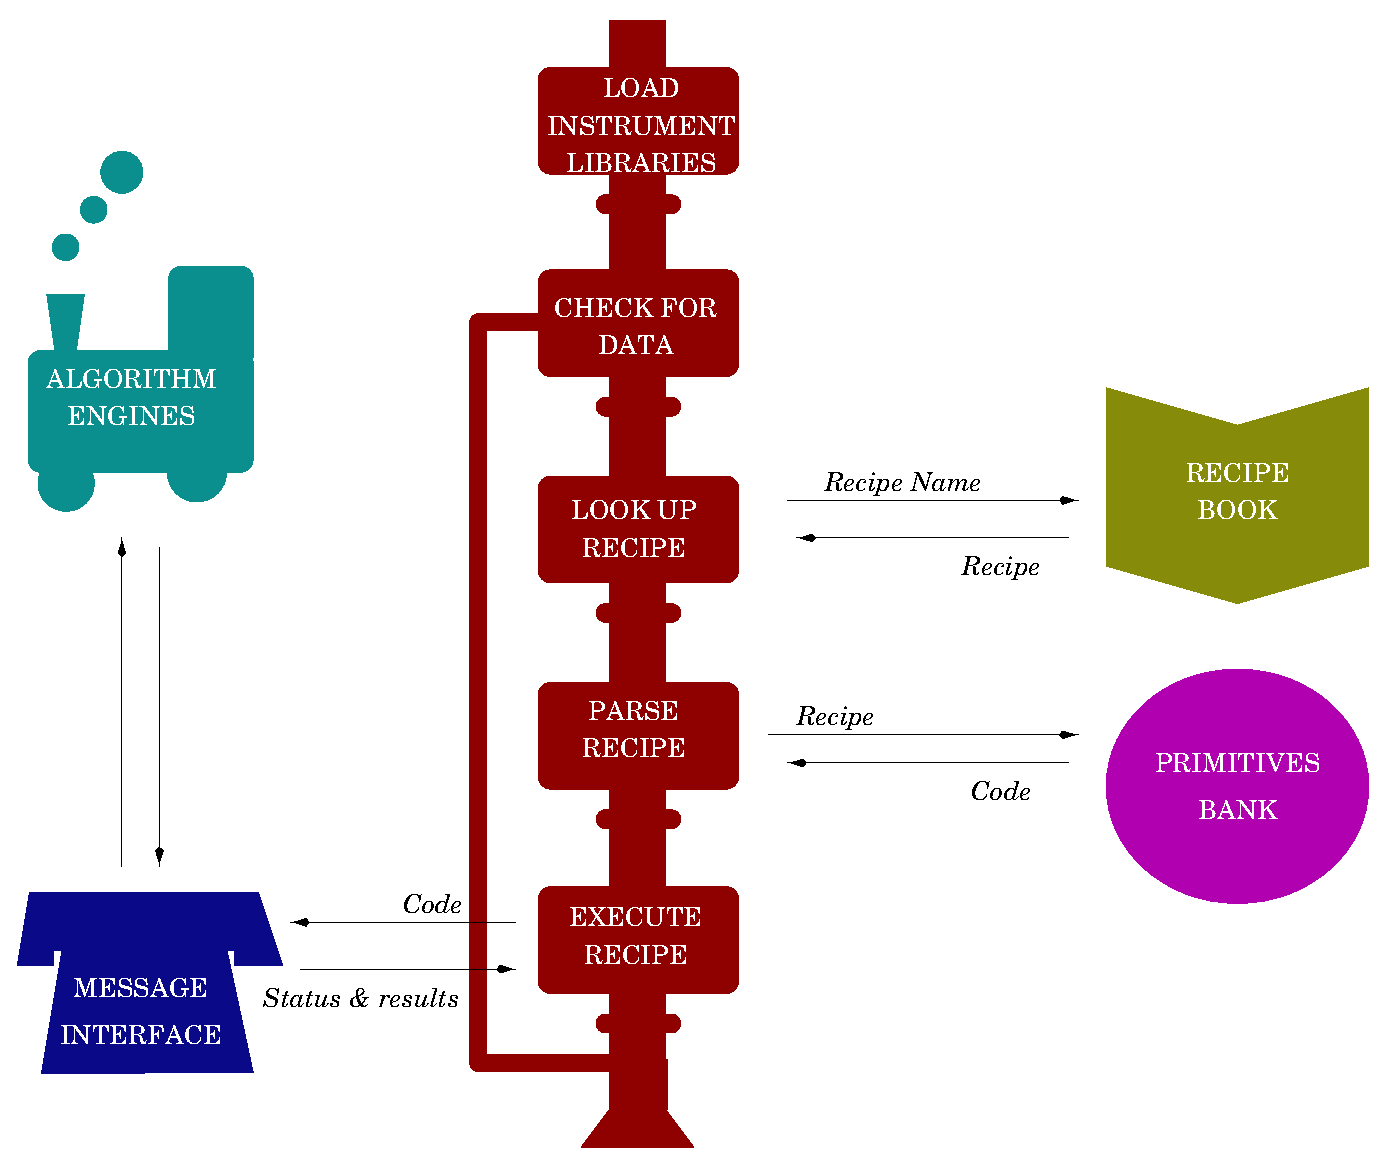
\includegraphics[width=\textwidth]{sun233_train.eps}
\caption{Outline of the modularity of ORAC-DR}
\label{fig:train}
\end{figure}

This document provides information on writing recipes and for adding
support for new instruments to the pipeline.


\section{Recipes}

Recipes in \Oracdr\ consist of a series of data reduction steps
(primitives) containing instructions for the reduction of
data. In general, recipes are different for each instrument supported
and are keyed to the specific observing mode used to take the data.

An example recipe may look something like:

\begin{myquote}
\begin{verbatim}
=head1 NAME

RECIPE_NAME - Short description of what the recipe does

=head1 DESCRIPTION

Long description of what recipe does.

=head1 NOTES

Some notes associated with the recipe.

=head1 SEE ALSO

List of related recipes.

=head1 AUTHORS

List of authors

=cut

_INSTRUMENT_HELLO_
# A comment
_STEP_ONE_
_STEP_TWO_  ARG1=number ARG2=string
_STEP_THREE_
_TIDY_RECIPE_
\end{verbatim}
\end{myquote}

This recipe illustrates all the important features of a recipe:

\begin{itemize}
\item The recipe must contain documentation in the Perl POD syntax
(see e.g.\ the \textsc{perlpod} manpage). This documentation is used
by the \oracman\ command and for the automated documentation system.
At the very least, recipe documentation should include \textbf{NAME}
and \textbf{DESCRIPTION} fields. The \textbf{NAME} field should use
the standard Perl format of
\begin{myquote}
\begin{verbatim}
RECIPE_NAME - purpose
\end{verbatim}
\end{myquote}
so that the POD translators can correctly determine this information
when generating \latex\ and HTML code.

\item To simplify the readability of recipes for non-programmers and
to separate the recipe language from the programming language
used to implement the primitives, no computer code should be visible
in the recipe.\footnote{\Oracdr\ does not \emph{enforce} this rule
though and it is possible to include Perl constructs in private
recipes and for testing. It should not be done for production code.}

\item Recipes are in plain text and are easily edited by support
scientists and users with the aid of a text editor. This also means
that is should be easy to support a GUI based drag-and-drop-type
recipe builder at a future date.

\item For most instruments, it is required that a \textbf{HELLO}
primitive be included at the start of every recipe. This is used 
to guarantee that steps certain initialization steps are always
executed. See individual instrumentation documentation to see whether
a \textbf{HELLO} primitive is required.

\item The comment character is a \#. All text after a \# is ignored by 
the recipe parser.

\item Configuration options can be passed into primitives by the use
of a \texttt{KEYWORD=value} string. The recipe parser automatically
converts these values into arguments suitable for the primitives.


\item A \textbf{TIDY} primitive is required at the end of most
recipes. This can be used to remove intermediate files at the
end of a recipe and any other tidying operation Usually calls the
\primitive{\_DELETE\_TEMP\_FILES\_} primitive. It must make sure that
files are not deleted that are subsequently required for group processing.


\end{itemize}

\subsection{Recipe Names}

The names of recipes should be descriptive. Short obtuse names are not
recommended since it should be obvious to the observer which recipe is
associated with which observing mode. In general, recipe names are
read from the file header, the location of which is specified by the
instrument specific classes in the \Oracdr. If required though, the
recipe can be specified on the command line although this can cause
problems if the user specifies the wrong observation numbers.

\subsection{Recipe locations}

\Oracdr\ searches in two locations for the recipe files. First, the
directory specified by the \texttt{ORAC\_\-RECIPE\_DIR} environment
variable, if defined, is searched. This allows users of the pipeline
to modify a standard recipe without editing the original. If the
variable is not set or the recipe can not be found, the default
location of \texttt{ORAC\_DIR}/recipes/\texttt{ORAC\_INSTRUMENT} is
searched (although \oracdr\ can sometimes be used to modify the value
of
\texttt{ORAC\_INSTRUMENT} during initialization). The pipeline
aborts if the recipe can not be located.



\section{Primitives}

\Oracdr\ primitives contain for the manipulation of data in a
given state. They are written using object oriented techniques,
manipulating objects associated with the individual data frames as
well as groups of observations. The steps that involve actual
processing of data (as opposed to housekeeping etc tasks) are done via
a messaging request to an algorithm engine resident in memory.

Because primitives always manipulate objects associated with the
pipeline, they are order-ignorant, i.e.\ no assumptions are made about
the file number, file name, or filename convention. These behaviours
are all handled by instrument-specific classes, thus allowing the
possibility of changing these conventions for an instrument without
changing code and of re-use of primitives elsewhere in different
recipes for different instruments.

Additionally, it is possible for primitives to contain instructions to
include other primitives. No limit is given on the number of
primitives that can be included (or the inclusion) depth but care must 
be taken to avoid recursion since, currently, the recipe parser will
simply continue reading in the primitive until the process runs out of 
memory! The recipe parser recognises primitive inclusion directives
by matching the pattern \verb|^\s*_|, ie an underscore as the first
blank character on a line. The primitive directive should look exactly 
as it would if found in a recipe, i.e.:
\begin{myquote}
\begin{verbatim}
 _SOME_PRIMITIVE_ ARG=arg  ARG2=$a  ARG3=$b
\end{verbatim}
\end{myquote}
and not
\begin{myquote}
\begin{verbatim}
 _SOME_PRIMITIVE_(ARG=arg,ARG2=$a, ARG3=$b);
\end{verbatim}
\end{myquote}
as would normally be expected for Perl. One difference from the recipe 
level\footnote{purely becaues the recipe level does not contain code} is that
perl scalar variables can be used to pass values into the primitive
rather than having to hard-code a specific value. The current recipe
parser does not yet allow complex data structures (arrays, hashes,
objects, references) to be passed into primitives. This is because
of a desire to enforce simple interfaces to all primitives regardless
of location rather than an inability of the parser to be modified to
support it, if there is demand for it, this feature could be added.

The following variables are available to all primitives:

\begin{description}
\item[\$Frm] \mbox{} % $

  Object of class \texttt{ORAC::Frame} (or a subclass thereof). This
object contains information about the \emph{current} frame being
processed by the pipeline. Methods are provided for accessing the
current filename and the header information.

\item[\$Grp] \mbox{} % $

Object of class \texttt{ORAC::Group} (or a subclass thereof). This
object contains information about the \emph{current} group being
processed by the pipeline. In \Oracdr\ a group is thought of as an
array of frame objects. Methods are provided for accessing the current
filename and current group members. The current frame will be a member
of the current group. The usual behaviiour is that the group object
will contain the frames processed so far that are part of the group,
in which case the last member of the group is the current frame.
Alternatively, it is possible for the group object to know about all
members of the group regardless of which have been processed already,
in which case the current frame may not necessarily be the last frame of
the group. The latter behaviour is controlled by the \texttt{-batch}
switch in \oracdr\ and can be used by primitive writers to delay group 
processing until the current frame is the last member of the group (a
group method is provided to determine this). This is only relevant for 
processing off-line but can significantly reduce run time of certain
recipes. Currently, SCUBA is the
only instrument that supports the batch option.

\item[\$Cal] \mbox{} %$

This provides access to the instrument's calibration system. This object
can return information such as the dark and flats to use for infrared
data or the current sky opacity for SCUBA. Extensive use is made of
index files and some primitives and recipes  must be responsible
for filing calibration data with this object so that later recipes
can access the correct information. The behaviour of this object is 
completely instrument specific, in general very few methods are
inherited by subclasses.

\item[\$Display] \mbox{} % $

An object of class \texttt{ORAC::Display}. Used by primitive writers
to send data display commands to the display subsystem. Note that
sending a display command does not necessarily result in anything
being displayed. The display system itself is not discussed in this document
[see the internals document].

\item[\%Mon] \mbox{}

A hash containing \texttt{ORAC::Msg} objects. These objects are used
to send messages to the algorithm engines. The hash keys will describe 
which algorithm engine is to be contacted. The instrument interface
should describe which tasks are available to programmers. Methods are
provided to send messages to algorithm engines (always waiting for the
reply before continuing) and for retrieving parameter values.

\item[\$ORAC\_PRIMITIVE] \mbox{} % $

This is the name of the current primitive. Usually used for debug
messages. Since this variable has a scope of the current primitive
only, if other primitives are included from within a primitive 
a new variable will be defined in the scopre of the included
primitive. This will generate warnings if the \texttt{-w} switch
is turned on since the current variable will mask the variable defined
in the scope of the parent primitive (as desired).


\item[\%\_PRIMITIVE\_NAME\_] \mbox{}

Hash containing the arguments available to the current primitive. The
name of the hash is the same as the name of the primitive (i.e.\ the
hash is not named \texttt{\_PRIMITIVE\_NAME\_} explicitly).

\end{description}

All primitives (and in fact all of \Oracdr) are written with the 
\texttt{strict} pragma turned on (see \texttt{perldoc strict} for more 
information) primarily to force a declared scope for all variables.
All primitives are evaluated by the Perl interpreter as
\begin{myquote}
\begin{verbatim}
preamble added by the parser
{
  preamble added by the parser in limited scope
  _PRIMITIVE_
}
\end{verbatim}
\end{myquote}
such that each primitive is in a different block to all other
primitives\footnote{unless the primitive is nested inside another
primitive}. The only global variables used by primitives should be
those supplied by the pipeline, all other variables should be lexical
(i.e.\ using the Perl \texttt{my} declaration) and will therefore be
freed at the end of the primitive. Passing complex information between 
primitives must be achieved by other means and is discussed in
\S\ref{information_passing}. 

All recipes are evaluated in the \texttt{ORAC::Basic} namespace.
This fact should not be used by any primitives and it is not
guaranteed that this namespace will be used in future releases 
of \Oracdr. It can always be assumed that functions and methods from the
following modules will be visible to all primitives:

\begin{description}
\item[ORAC::Print] \mbox{}

Provides the \texttt{orac\_print}, \texttt{orac\_err} and
\texttt{orac\_warn} commands. These routines route messages to 
the correct output systems (an X-window, the screen, a log file etc)
specified by the user. The standard perl functions \texttt{print} and
\texttt{warn} should not be used for user messages except during
development since the user has no control of where to send them.

\item[ORAC::LogFile] \mbox{}

Used to write log files (see \S\ref{logfiles}).

\item[ORAC::Constants] \mbox{}

Provides access to the standard \Oracdr\ constant. The most important
are \texttt{ORAC\_\_OK} and \texttt{ORAC\_\_ERROR} (note that they 
are Perl constants, not variables).

\item[ORAC::TempFile] \mbox{}

Use to generate temporary files (see \S\ref{tempfiles}).

\item[ORAC::General] \mbox{}

Functions that are usuful but are not necessarily a standard part of
Perl. Examples are \texttt{max()}, \texttt{min()} and \texttt{log10()}.

\end{description}


\section{Writing a Primitive}

In order to write a valid primitive certain steps must
be adhered to in order to ensure that subsequent primitives
have the correct information.

It assumes knowledge of the following Perl concepts:
using Perl objects, lexical variables, Perl data
structures. 

Here is an example primitive showing the basic princples:

\begin{myquote}
\begin{verbatim}
 1  =head1 NAME
 2
 3  _PRIMITIVE_NAME_ - short description
 4
 5  =head1 DESCRIPTION
 6 
 7  Long description
 8
 9  =head1 ARGUMENTS
10
11  =over 4
12
13  =item ARG1
14
15  Description of possible values of ARG1
16
17  etc...
18
19  =back
20
21  =head1 TASKS
22
23  List of external tasks required by the primitive
24
25  =head1 OUTPUT FILES
26
27  Output suffix for the display system.
28
29  etc, AUTHORS, COPYRIGHT.....
30
31  =cut
32
33  # Read arguments or use default values
34  my $arg1 = ( exists $_PRIMITIVE_NAME{ARG1} ? 
35               $_PRIMITIVE_NAME{ARG1} : 5);
36
37  # Loop over all sub frames
38  foreach my $i (1..$Frm->nfiles) {
39
40    # Get the input and output filename
41    my ($in, $out) = $Frm->inout('_sfx', $i);
42
43    # Read some value from the frame FITS header
44    my $value = $Frm->hdr('KEYWORD');
45
46    # Combine the in, out and value into options for the task
47    # DEPENDS ON ALGORITHM ENGINE
48    my $options = "IN=$in OUT=$out SWITCH=$value";
49
50    # Run the algorithm engine
51    $Mon{'task'}->obeyw('TASK',$options);
52
53    # Retrieve an answer from a parameter
54    ($ORAC_STATUS, $result) = $Mon{'task'}->get('TASK','PARAMETER');
55
56    # Print the result
57    orac_print "Result from primitive $ORAC_PRIMITIVE = $result\n";
58
59    # Update the frame object so that the next primitive
60    # gets the correct input file name
61    $Frm->file($i, $out);
62
63  }
64
65  # Ask the display system to display the frame
66  $Display->display_data($Frm) if defined $Display
67
\end{verbatim}
\end{myquote} %$
The following should be noted:
\begin{itemize}

\item Primitives are written in Perl and all variables are lexicals
(using \texttt{my}).

\item As for recipes, the first few lines (1--31) are the
documentation for the primitive in pod format. In addition to the
fields used for recipe headers, three new fields are required for
primitives, \textbf{ARGUMENTS} to describe the configuration options,
\textbf{TASKS} to list external dependencies and \textbf{OUTPUT FILES}
to list the suffix of any output data files (for use with the display
system) and any log files that may be written.

\item Supplied arguments can be read from the \_PRIMITIVE\_NAME\_
hash. Lines 33--35 check for the existence of the \texttt{ARG1}
key in the hash and read it if it exists else a default value is
copied in. Note the use of \texttt{exists} rather than
\texttt{defined} for checking hash contents. If \texttt{defined} is
used the key would automatically be created in the hash and set to a value of
\texttt{undef} whereas \texttt{exists} simply looks for the key in the 
hash without creating it. In general, this is the more correct
behaviour as it can distinguish between the key not being there at all 
(i.e.\ never set) and the key being set explicitly to
\texttt{undef}\footnote{Although it is not possible for a user to
specify a primitive argument value of \texttt{undef} this is still
good programming practice}

In some current primitives the following may
be found for reading arguments:
\begin{myquote}
\begin{verbatim}
my $arg1 = ( $_PRIMITIVE_NAME_{ARG1} || $default);
\end{verbatim}
\end{myquote} %$
This works in most normal cases but will fail if the value of the
argument is desired to be `0' since that evaluates to false and will
cause the default to be returned rather than a `0'. This construct
also causes the key to be created even if no argument was ever
supplied (known as \emph{auto-vivification}).

\item Line 38 starts a loop over all the sub-frames present in the
frame. The need for such a loop depends on the individual instrument.
UFTI, for example, only ever creates a single data frame per disk file
and so will not require the loop. SCUBA can take data for multiple
wavelengths, and MICHELLE can store multiple integrations per dat
file, so this loop would ensure that each wavelength/integration is
processed in turn.

\item Line 41 retrieves the name of the current input file and
supplies a valid output filename based on the supplied suffix. Note
that this command accepts a number as an optional argument. This 
can be used to connect the file name with the sub-frame (a Frame
object can store multiple current filenames).

\item Line 44 simply retrieves a value from the header. The
\texttt{hdr()} method can also be used to set header values (but does
not change the header on disk).

\item Lines 46--51 send a message to an algorithm engine using a
messaging object stored in the \texttt{\%Mon} hash. The options
string depends on the task at the other end of the message bus and
will therefore need to be changed if the algorithm engine is changed.
An important point is that error checking code is automatically
inserted into the recipe when  \texttt{$->$obeyw} is found in a line
that is not preceeded by an equals sign or a comment. This means that
line 51 is translated to:
\begin{myquote}
\begin{verbatim}
{
  my $OBEYW_STATUS = $Mon{'task'}->obeyw('TASK', $options);
  if ($OBEYW_STATUS != ORAC__OK) {
     < ERROR MESSAGE CONSTRUCTED AND PRINTED WITH orac_err>
     return $OBEYW_STATUS;
  }
}
\end{verbatim}
\end{myquote} %$
such that the recipe is aborted and an error message printed. Note
that this block runs in its own scope to prevent warnings from Perl
concerning the masking of previous \texttt{OBEYW\_STATUS} variables.

If automatic checking is not required, simply check the return
status. If the parser finds an equals sign before the \texttt{obeyw}
the line will not be re-written.

\item Line 54 retrieves an parameter value from the external task.
This example also makes use of the automatic status checking within
\Oracdr. Whenever the parser sees the special \texttt{ORAC\_STATUS}
variable in a primitive, code is automatically after this line to
check the value of \texttt{ORAC\_STATUS} and compare it against
\texttt{ORAC\_\_OK}. If status is not good, the recipe aborts and an
error message is printed. This saves the primitive writer from having
to worry about status checking.

\item Line 57 makes use of the \texttt{orac\_print} command to send a
message to the user. The \texttt{orac\_print} command is written to
send the message to multiple output filehandles as defined by the user 
with the \texttt{-log} switch to \oracdr.

\item The final task in the loop (line 61 ) is to update the file name
stored in the frame object. This step is viatal, and without it subsequent
primitives will use the wrong input file name. 

\item The final step is to display the reduced frames. The
\texttt{display\_data} method will ask for the current frame to be
displayed. Note that the display sub-system will \emph{only} display
the data frame if the user has requested this by configuring the
display system (using, for example, the \texttt{oracdisp} command)
accordingly. The check to make sure the display object is initialised
is required in case the user has turned off the display system.

\end{itemize}

\subsection{Log Files\label{logfiles}}

It is sometimes desirable to write results to log files as data
files are processed (for example, seeing statistics, pointing offsets
etc). Rather than force the primitive writer to check for the
existence of log files and decide whether or not to open or append to
log files, the \Oracdr\ system provides a simplified access to log
file creation via the \texttt{ORAC:LogFile} class.

All that is required to write an entry to a log file is for the
following methods to be invoked:
\begin{myquote}
\begin{verbatim}
my $log = new ORAC::LogFile('log.whatever');
$log->header(@header);
$log->addentry(@lines);
\end{verbatim}
\end{myquote} %$
The header will only be written to the log file if the log file
does not previously exist so it is safe to run this command in a
primitive without an explicit check. Both the \texttt{header()} and
\texttt{addentry()} methods accept arrays and newline characters will
be appended to each item in the array when written to the log file.
The convention is that all log file names should start with `\texttt{log.}'.

\subsection{Temporary and intermediate files\label{tempfiles}}

In many cases, it is necessary to make use of temporary files
within a primitive, either for intermediate data steps that are not
relevant for the frame or text files as input to external tasks. Since
these are not required once the primitive is finished a class is
provided for dealing with temporary files (\texttt{ORAC::TempFile}).

This class will choose a filename and, optionally, open the file ready 
for read-write (when this facility is used it is guaranteed that the
file is unique and will not overwrite any existing file). The file,
and any files of the same name but with a \texttt{.sdf}
extension\footnote{the extension used for Starlink N-Dimensional data
format (NDF)}, are removed when the variable goes out of scope.

The only files that should remain when a primitive completes should be
those registered with the current frame or the current group. All
others should be temporary and should be tidied up on leaving the
primitive (which is automatic if \texttt{ORAC::TempFile} is used.
This allows the final tidyup primitive to be responsible solely for
removing unwanted intermediate files that were the product of
individual primitives (every time a the file name is updated in a
frame object the previous value is stored for possible later removal
by the tidy primitive). 

\subsection{Passing information between primitives\label{information_passing}}

Since each primitive is evaluated in its own scope, it is not possible 
(or even desirable) to pass simple variables between separate
primitives. Two means are provided for doing this:

\begin{itemize}
\item Using the \texttt{\%\_PRIMITIVE\_NAME\_} hash. The argument hash 
for each primitive is visible to all other primitives at the same
level. This works but has a number of problems:
\begin{itemize}
\item The system breaks if the previous primitive is removed from the
recipe.\footnote{It will not simply return \texttt{undef}. The recipe
will fail to run since the hash would not have been declared previously.}
\item The system breaks if the primitive is renamed
\item If the primitive from which data are required is in a different
scope from the current primitive this will not work.
\item It feels too much like a global variable.....
\end{itemize}

\item Store the information with the current frame or group object.
Both frame and group objects can use the \texttt{uhdr()} method to
store arbritrary data (including references) in a hash. This is the
recommended way of transferring data between primitives when the
information relates to the current frame or group. By convention, the
\texttt{hdr()} method should be used for storing FITS-like data.
Checks should be made for the existence of data in the hash before
using it.
\end{itemize}


\section{Calibration}

The calibration system is essentially based on the concept of index
files.  An index file is a data file containing information on all
calibration observation reduced by the pipeline. A separate index file
is created for each calibration sub-system (e.g.\ one for dark
observations, one for skydip observations etc) with the convention is
that each index file is stored in \texttt{ORAC\_DATA\_OUT} and
prefixed with the string \texttt{index.} (e.g.\ \texttt{index.dark},
\texttt{index.skydip} etc). It is the responsibility of a primitive
(usually a complete recipe is dedicated to the calibration
observation) to file a calibration to an index file. The index file
can be used simply to register a file name (e.g.\ the name of a dark file
or flatfield) or a calibration result (the current sky opacity or flux
conversion factor). Methods are provided in the \texttt{ORAC::Index}
class for retrieving this information from the index file\footnote{For
efficiency, the index file is kept in memory rather than read from
disk every time it is to be accessed. This means that \Oracdr\ is not
guaranteed to work if two processes are sharing a single ouput data
directory as this would cause problems with index file updates [they
are not locked].}

The index object is responsible for searching the relevant index
file and returning the most suitable calibration. This is achieved by
the use of external rules files (stored in \texttt{ORAC\_DATA\_CAL}
called \texttt{rules.CALIBRATION\_NAME}) which list which header
keywords are relevant and should be checked against the headers of the
current frame. This means that the calibration object itself does not
need to worry about searching the index file or reading the rules
files. 

An example rules file could look like:
\begin{myquote}
\begin{verbatim}
# Example rules file for SCUBA skydips
MODE eq 'SKYDIP'
FILTER == $Hdr{FILTER}
TAUZ
ORACTIME ; abs(ORACTIME - $Hdr{ORACTIME}) < 0.5
\end{verbatim}
\end{myquote}

The format is intended to be fairly simple as it should be possible
for a non-programmer to edit it. The main points are:

\begin{itemize}
\item \# is the comment character. Anything after a comment is
ignored.
\item Blank lines are ignored
\item Each line in the rules file is translated to the Perl code and
evaluated. If it returns `true' the value in the index file (keyed by
the first word in the rules file) matches the coresponding values in
the header of the current frame. For example, the last line in the
above rules file could be translated to the following if (using
ORACTIME of 19990827.55 for the index entry):
\begin{myquote}
\begin{verbatim}
'19990827.55'; abs(19990827.55 - $Hdr{ORACTIME}) < 0.5 
\end{verbatim}
\end{myquote} %$
which returns true if the \texttt{ORACTIME} stored in the index is
within half a day of the value stored in the current frame object
(\%Hdr is a hash read from the current frame header).
The semi-colon is used to separate the Perl code into two statements.
The return value of the eval is that of the second statement. This is
required for cases that are not simply `\texttt{A == B}' format.
\item Lines which only contain a keyword, are placeholders indicating
that the information should be present in the index file but not used.
\end{itemize}

\section{Recipe debugging}

Some facilities are provided to ease the debugging of recipes and
primitives. These are:

\begin{itemize}

\item When a recipe will not compile (due to syntax errors for
example) the pipeline aborts and the error message and a listing of
relevant recipe lines (the version of the recipe executed internally
with all the extra code inserted) is printed to the screen.

\item The \texttt{-w} switch should be used during development 
in order to trap and fix any warnings detected by the Perl interpreter
at runtime. In many cases, these warnings are indicative of code that
makes assumptions about state (warnings on use of \texttt{undef}) or
scope (\texttt{my} declarations masking variables defined in a higher
scope). 

If warnings are raised from the \Oracdr\ core please contact the
authors and they will be fixed.\footnote{currently the one known issue 
is multiple declarations of the \texttt{ORAC\_PRIMITIVE} variable.}

\item The \texttt{-verbose} switch can be used to turn on messages from 
the algorithm engines. This is sometimes useful to make sure that the
external task is doing the expected operation.

\item The final option is to turn on full debugging with the
\texttt{-debug} switch. This creates a file in
\texttt{ORAC\_DATA\_OUT} called \textit{ORACDR.DEBUG} containing the
contents of each message sent to external tasks with an
\texttt{obeyw}. This can be used to find out what the final message
sent to a task was before the recipe crashed. Additionally, if a
recipe crashes when the debugging is turned on the full contents of
the recipe buffer (i.e.\ the fully parsed recipe) will be written 
to a file in \texttt{ORAC\_DATA\_OUT} called
\textit{ORACDR\_RECIPE.dump}.

\end{itemize}

The perl debugger should be used with care since it is possible to
hang the message bus if the program is frozen during a message
transaction and the debugger is not optimized for use with the use of nested
\texttt{eval} common in the pipeline internals.

A recipe checker is planned that will allow syntax to be checked
without having to load the entire \Oracdr\ system.

\section{Adding new instruments}

Adding a new instrument to \Oracdr\ requires a number of steps, the
complexity of which will depend on how close the instrument is to an
instrument that is already supported by the pipeline.

This section describes the areas that must be modified to support a
new instrument. It assumes knowledge of the following Perl concepts:
writing object oriented modules, lexical variables, Perl data
structures and \texttt{eval}. Message system interfaces will also
require a knowledge of Perl XS.


\subsection{Frames}

An \texttt{ORAC::Frame} class is responsible for filename conventions
and handling of sub-frames. The most common methods that need to be
subclassed are:

\begin{description}
\item[new()] \mbox{}

The object constructor should be modified to set the default behaviour
for \texttt{rawfixedpart()}, (the part of the filename that does not
change with UT date of observation number), \texttt{rawsuffix()},
(the file suffix of the raw data file),
\texttt{rawformat()} (the input format of the data: FITS, NDF etc)
and \texttt{format()} (the data format required by the algorithm
engines).

The base constructor (\texttt{SUPER::new()}) should be invoked to
instantiate the object.

\item[calc\_orac\_headers()] \mbox{}

This method is used to translate instrument specific headers to those
required by the pipeline. Currently this method must insert the
following  keywords into the frame header:

\begin{description}
\item[ORACUT] \mbox{}

This should be the UT date of the observation in YYYYMMDD format.

\item[ORACTIME] \mbox{}

This should be the UT date and time of the observation in
YYYYMMDD.frac format (i.e.\ UT date plus fraction of day). This is
used by the calibration system to ensure that a guaranteed time stamp
can be used for comparison in index files.

\end{description}

\item[file\_from\_bits()] \mbox{}

Given a UT date  and an observation number return the name of the 
raw data file. This is used by the pipeline to look for the file on disk.

\item[flag\_from\_bits()] \mbox{}

Given a UT date and an observation number, return the name of the flag 
file. This is used by the pipeline to search for a completion flag on
disk associated with the current observation file. Only required if 
it is intended for the pipeline to be used in conjunction with the 
\texttt{-loop flag} option.

\item[findgroup()] \mbox{}

Translates the header values into a group name and update the frame.

\item[findrecipe()] \mbox{}

Translates the header values into a recipe name and update the frame.

\item[template()] \mbox{}

Modifies the current filename so that it matches the filename that you 
would have had had at an earlier point in the reduction when the
supplied template was valid. This is used for jumping to earlier steps
in the reduction when performing group operations.
Currently this method is generally
implemented by replacing the suffix with the supplied value. It could
also be implemented by accessing the list of prior file names with the
\texttt{intermediates()} method.

\item[inout()] \mbox{}

Given a suffix and sub-frame number provide a recommended name for the 
output file. Does not update the frame object. In general, this can
either simply append the suffix or replace the last suffix.

\end{description}

In addition to those listed above, some methods need to know something
about the file format and should be modified (most UKIRT and JCMT
instruments inherit from the \texttt{ORAC::Frame::NDF} class rather
than \texttt{ORAC::Frame} since that class knows how to read from NDF
files). The automatic format conversion will have occurred before
these methods need to be run (for example if the input format is FITS
but the processing format is NDF, then the methods should be written
assuming NDF files). These methods are:

\begin{description}

\item[readhdr()] \mbox{}

Reads the file header and stores the resulting hash reference in the
object. Also forces the ORAC headers to be calculated.

\item[erase()] \mbox{}

A method to delete the file currently associated with the frame. This
is effectively and \texttt{unlink()} but for NDF files the
\texttt{.sdf} is appended. The base class implementation can be used
in most cases.

\item[file\_exists()] \mbox{}

Checks to see if the data file exists. A special case for NDF format
since the \texttt{.sdf} extension is not present in the file name.

\item[stripfname()] \mbox{}

Strips the extension from the filename. The base class does nothing to 
the filename.

\end{description}

Finally, any extra methods not present in the base class but required
by an instrument should also be added. These can cover translation of
wavelengths to sub-frame filenaame for example (used by the SCUBA class).


\subsection{Groups}

An \texttt{ORAC::Group} class is responsible for dealing with groups
of frame objects and with an output group data file.
The most common methods that need to be subclassed are:

\begin{description}

\item[new()] \mbox{}

The constructor must be overriden to specify the type fixed part and
file suffix of the ouptut group file. The base constructor should be
used from the subclass to instantiate the object.

\item[readhdr()/erase()/file\_exists()/file\_from\_bits()] \mbox{}

Similar to the frame implementations.


\end{description}

For specialized applications it may also be necessary to implement 
the \texttt{coaddswrite()}/\texttt{coaddsread()} methods. These will
be used by the CGS4/MICHELLE instrument classes to allow coadds to be 
combined part way through a group without having to re-reduce earlier
observations. Not all instruments require support for this.

\subsection{Calibration}

For a new instrument all that is required is to specify a new
set of rules and work out what to do with the `best' calibration that
is returned. For UFTI this simply means that the name is returned to
the primitive for use. For SCUBA more complex routines are required
for sky opacity calibration since the number returned by the index
file is sometimes modified for different filters before being returned 
to the user (the SCUBA calibration system never returns a file name).

For every type of calibration, the calibration object must provide the 
following methods:
\begin{enumerate}
\item A method for returning the current calibration observation that
matches the criteria. This method should be an obvious name related
directly to the calibration (e.g.\ `dark', `skydip').
\item A method for retrieving the \texttt{ORAC::Index} object
associated with the relevant index file. The name of this method
should be related to the name of the index file (e.g.\
\texttt{skydipindex} will access the file \texttt{index.skydip}).
\item A method to prevent the pipeline from overwriting the current
calibration (used when the user is overriding a certain calibration
from the command line). This will be called, for example,
\texttt{darknoupdate()}. \oracdr\ assumes that the method will assume
it is of this form since this method will be called whenever a user
makes use of the \texttt{-cal} switch,

\end{enumerate}



\subsection{Algorithm Engines}

Each instrument requires its own implementation of an
\texttt{ORAC::Inst} module. This module is responsible for
implementing the commands for starting the messaging layer (if
required) and launching external tasks ready for use by the
pipeline. It may be possible for future releases to launch
external tasks on demand the first time an \texttt{obeyw} is
issued but this depends on the implementation of the messaging class and 
still requires that an object for each class is instantiated in the
\texttt{ORAC::Inst} module at startup.

Currently, this module is not object-oriented. This may change in the
future.

Another factor related to the algorithm engines is the implementation
of the mesaging interface. Currently, an interface is provided to the 
ADAM messaging system used by Starlink. An additional interface is
provided to run ADAM tasks via the Unix shell as a proof of concept.
Interfaces to Glish and IRAF will be needed to talk to \textsc{aips++}
and \textsc{Iraf} tasks. A Perl to DRAMA interface exists and it
should be fairly simple to write an \Oracdr\ interface for
DRAMA tasks. A shell interface should be used as a last
resort and only if valid exit status can be returned to the pipeline.



\subsection{\oracdr}

Once the instrument classes have been written, \oracdr\ needs to be
modified so that it can interpret a new value for
\texttt{ORAC\_INSTRUMENT} and configure the frame, group and
calibration objects correctly.

In the future this configuration may be moved into an external data
file so that the core \oracdr\ routine need not be modified by people
porting the system to a new instrument.

\subsection{Recipes}

Once \Oracdr\ has been configured to recognise the new instrument, the 
final step is to write the recipes and associated primitives to deal
with the new data and possibly new algorithm engines. At its simplest, 
for example for an infrared image, this may simply require copying
pre-written primitives from an existing instrument\footnote{Plans are
ongoing to allow multiple search paths for recipes and primitives so
that single copies can be used by multiple instruments without having
to copy the files to separate locations}.
At its most complex, completely new primitives will have to be written.

\appendix

\section{Directory Layout}

\Oracdr\ is designed to include all its directories in a single
location and not to care where that location is. All \Oracdr\ software
is located relative to the directory described by  \texttt{ORAC\_DIR}
environment variable.

The standard layout is:

\begin{description}
\item[bin] \mbox{}

Executable programs. This includes \oracdr, \oracman\ and others. Note
that none of the programs that form part of \Oracdr\ are binary. 
The core \Oracdr\ system will run anywhere the necessary Perl modules
are available.

\item[recipes] \mbox{}

All the recipe files. Contains a directory for each instrument (using
upper case) usually matching the value of the
\texttt{ORAC\_INSTRUMENT} environment variable.

\item[primitives] \mbox{}

All the primitive files. Contains a directory for each instrument
(using upper case) usually matching the value of the
\texttt{ORAC\_INSTRUMENT} environment variable.

\item[howto] \mbox{}

Basic introductory documentation for \Oracdr.

\item[lib] \mbox{}

Library files required by \Oracdr. Contains a \texttt{perl5} directory
with all the Perl modules used by the system. The \texttt{perl5}
directory is the usual value for the \texttt{ORAC\_PERL5LIB}
environment variable.

\item[images] \mbox{}

Image files used by the system. Contains the start up images for the
display tools (in NDF format).

\item[docs] \mbox{}

Main documentation. Contains a directory per document. Currently
contains all the Starlink User Notes.

\item[gui] \mbox{}

Graphical user interface definitions. Only used by \oracdisp.

\end{description}


%%%%%%%%%


%%%% INSERT ShellVariables pod here

%%%%%%%%

\section{Core libraries}


\include{testpod}




% ? End of main text
\end{document}
